\section{Vector Extensions}

\begin{frame}{Array Programming}
\begin{itemize}
   \item Operations are exclusively done over vectors, matrices, and tensors instead of scalars
   \item Scalars in array programming are vectors with a single index
   \item Array programming simplifies programming linear algebra algorithms
   \item Array programming languages include MATLAB, Octave, R, Julia, and Python via NumPy
\end{itemize}
\end{frame}

\begin{frame}[fragile]{Array Programming in Python}
\centering\small
\begin{minted}{python}
>>> from numpy import matrix, linalg
>>> A = matrix([[1,2,3],[4,5,6],[7,8,9]])
>>> x = matrix([[1],[2],[3]])
>>> print(A.T)
[[1 4 7]
 [2 5 8]
 [3 6 9]]
>>> print(A*x)
[[14]
 [32]
 [50]]
\end{minted}
\end{frame}

\begin{frame}{Single Instruction, Multiple Data}
\begin{itemize}
    \item A single operation is applied to multiple data simultaneously
    \item Allows some linear alegra operations to be done via vectors instead of single elements
    \item Modern systems are MIMD where each processor or core can perform independent SIMD operations
    \item SIMD instructions are CPU architecture specific, \textit{i.e.}\ not all CPU's have the same SIMD instruction sets
\end{itemize}
\end{frame}

\begin{frame}[fragile]{Vectorization Example}
\centering
\begin{minted}{c}
for (int i=0; i<16; ++i) {
   C[i] = A[i] + B[i];
}

for (int i=0; i<16; i+=4) {
   addFourThingsAtOnceAndStoreResult(&C[i], &A[i], &B[i]);
}
\end{minted}
\end{frame}

\begin{frame}{Advanced Vector Extensions}
\begin{itemize}
    \item Advanced Vector Extensions (AVX) are a set of SIMD extensions to the x86 instruction set
    \item Initially developed by Intel in 2008
    \item Implemented in Intel and AMD CPU's since 2011
\end{itemize}
\end{frame}

\begin{frame}{AVX Versions}
\begin{description}
   \item[AVX]
    \begin{itemize}
        \item Expanded many of the earlier SSE floating point instructions from 128 to 256 bits
        \item Several new instructions
        \item Intel Sandy Bridge and AMD Bulldozer and newer architectures
    \end{itemize}
   \item[AVX2]
    \begin{itemize}
        \item Expanded many of the earlier SSE integer instruction from 128 to 256 bits
        \item Several new instructions
        \item Intel Haswell and AMD Carrizo and newer architectures
    \end{itemize}
   \item[AVX-512]
    \begin{itemize}
        \item Expanded AVX instructions from 256 to 512 bits
        \item Several new instructions
        \item Intel Xeon Phi x200 series CPU's
    \end{itemize}
\end{description}
\end{frame}

\begin{frame}{Vector Extension Widths}
\begin{center}
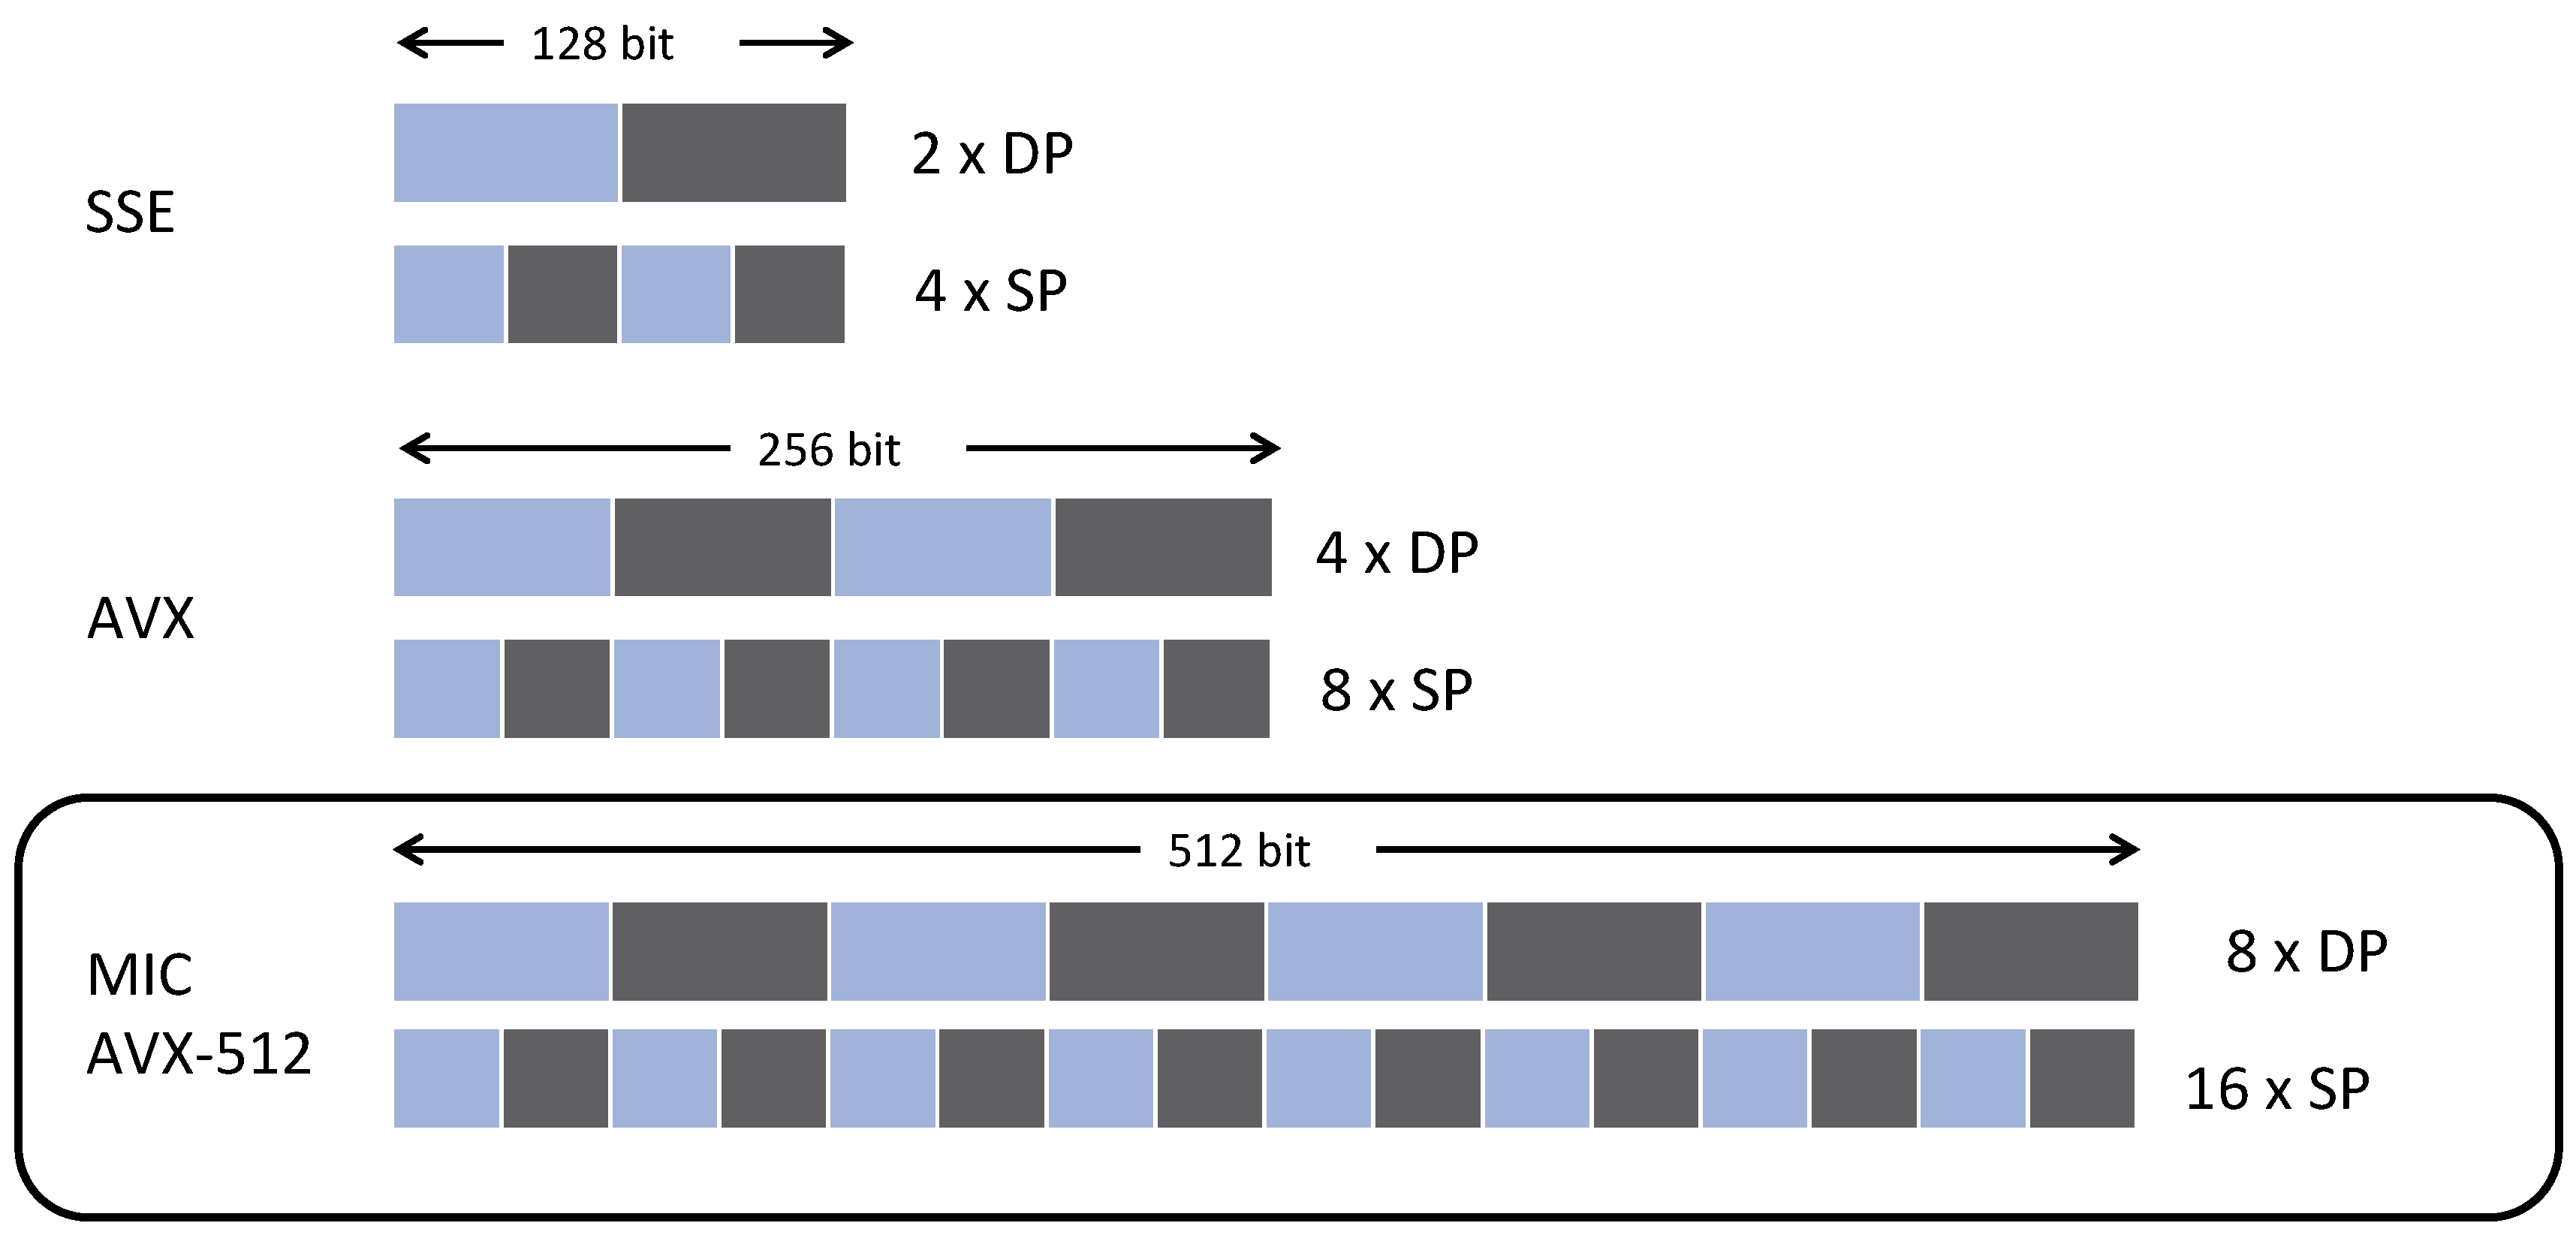
\includegraphics[width=\textwidth]{figures/vector_widths_1.pdf}
\end{center}
\end{frame}

\begin{frame}{Vector Extension Addition}
\begin{center}
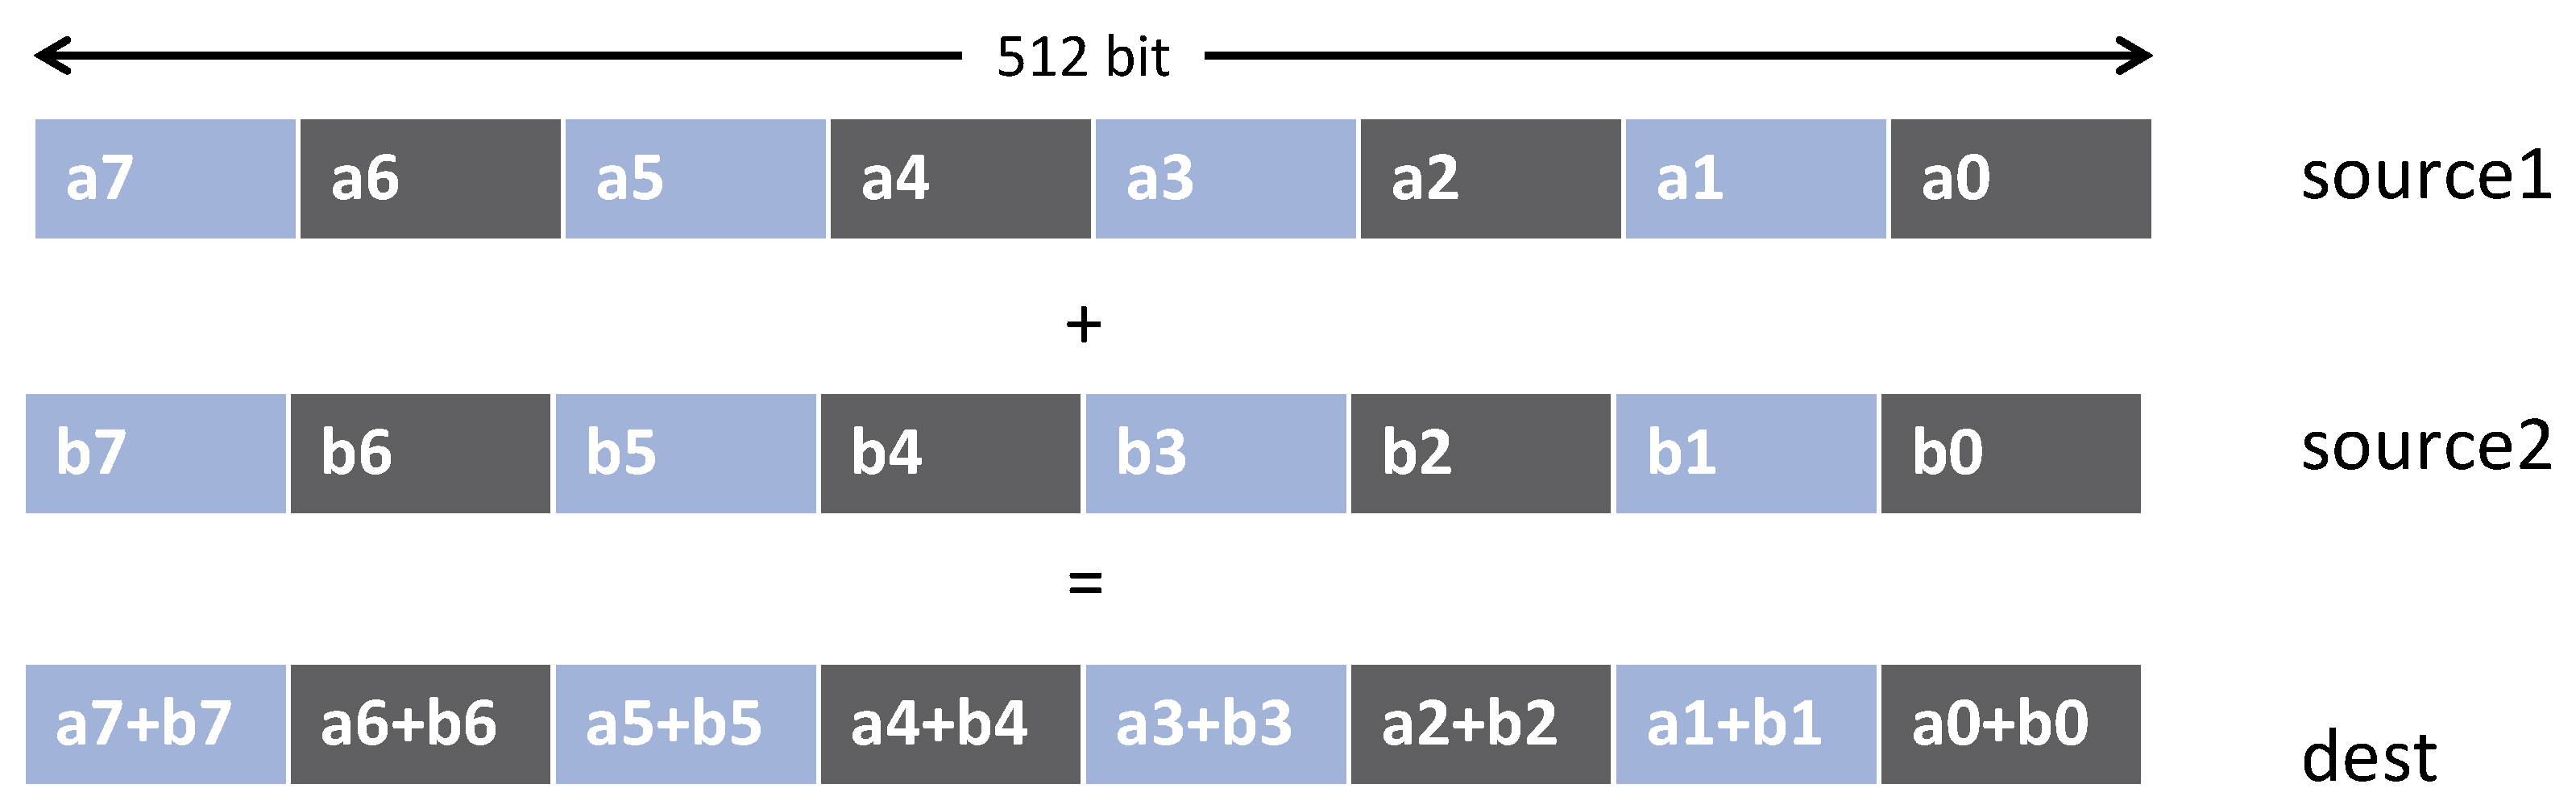
\includegraphics[width=\textwidth]{figures/vector_widths_2.pdf}
\end{center}
\end{frame}

\begin{frame}{Vector Extension Fused Multiply-Add}
\begin{center}
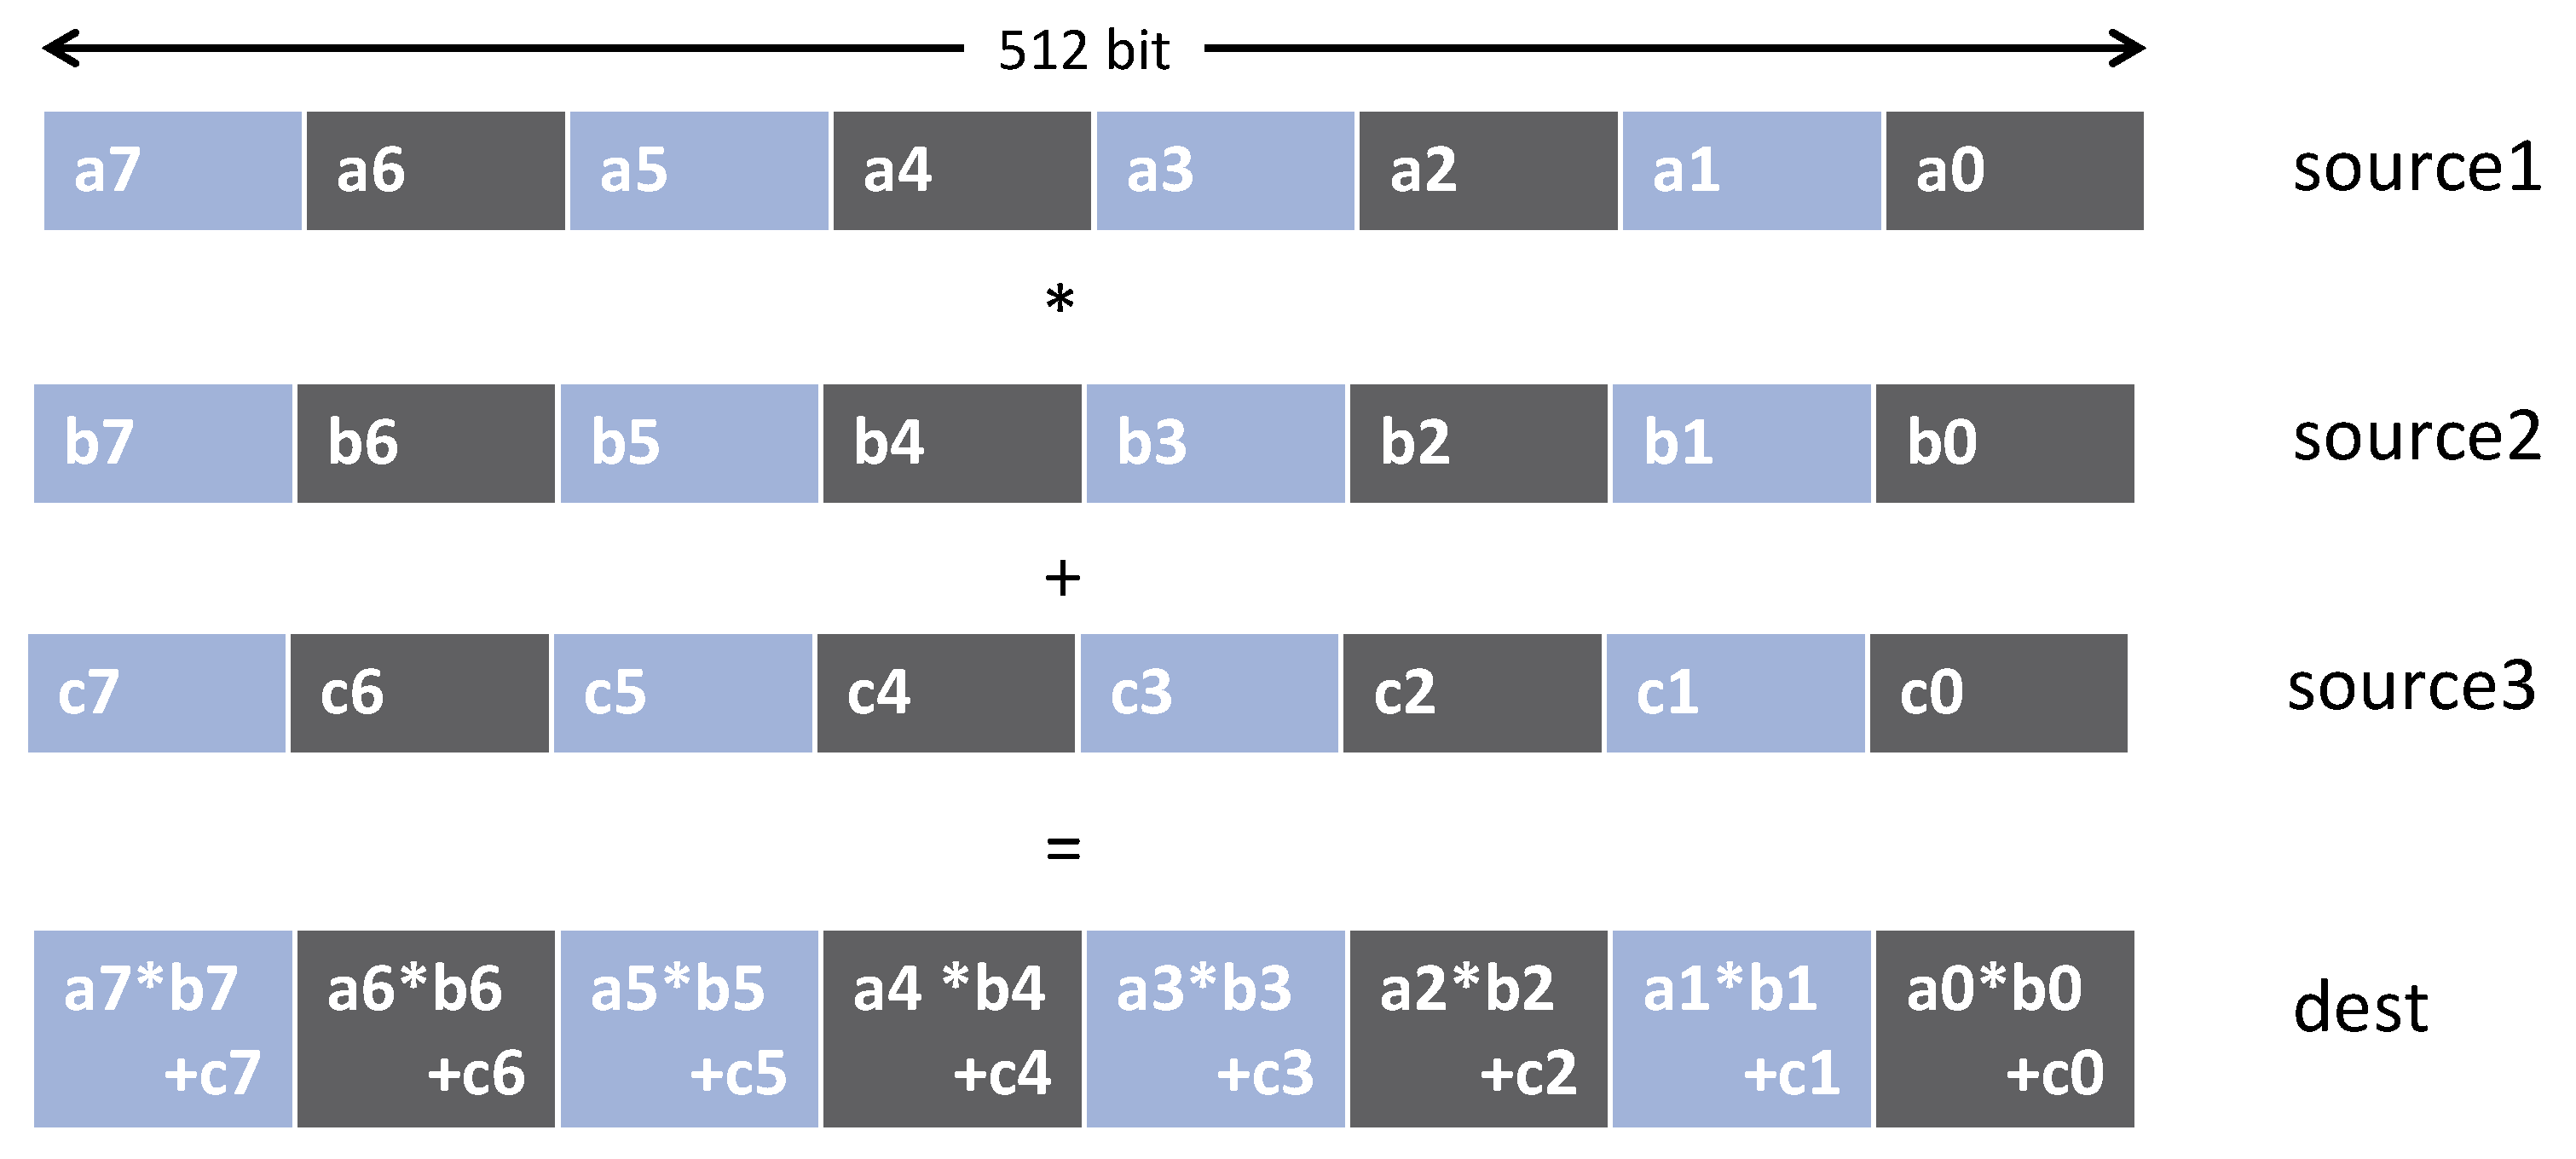
\includegraphics[width=\textwidth]{figures/vector_widths_3.pdf}
\end{center}
\end{frame}

